\documentclass[tikz,border=3mm]{standalone}
\usepackage{tikz}
\usetikzlibrary{angles,quotes,calc,intersections}
\begin{document}
% TikZ 1
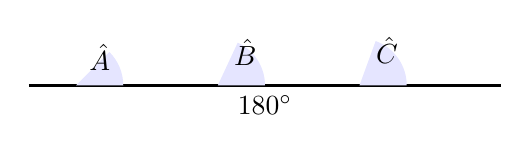
\begin{tikzpicture}[scale=1]
\draw[thick] (0,0)--(6,0);
\fill[blue!10] (0.6,0)--(1.2,0) arc[start angle=0,end angle=45,radius=.6]--cycle;
\fill[blue!10] (2.4,0)--(3.0,0) arc[start angle=0,end angle=65,radius=.6]--cycle;
\fill[blue!10] (4.2,0)--(4.8,0) arc[start angle=0,end angle=70,radius=.6]--cycle;
\node at (0.9,.35) {$\hat{A}$}; \node at (2.75,.42) {$\hat{B}$}; \node at (4.55,.45) {$\hat{C}$};
\node[below] at (3,0) {$180^{\circ}$};
\end{tikzpicture}
\hspace{1cm}
% TikZ 2
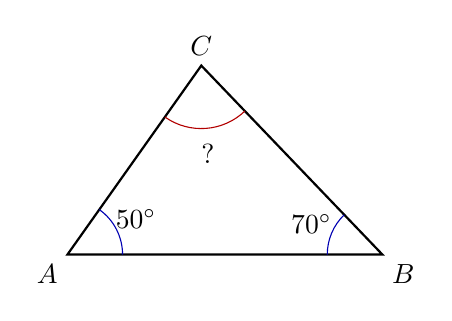
\begin{tikzpicture}[scale=1]
\coordinate (A) at (0,0); \coordinate (B) at (4,0); \coordinate (C) at (1.7,2.4);
\draw[thick] (A)--(B)--(C)--cycle;
\pic[draw=blue!70!black, "$50^{\circ}$", angle radius=7mm, angle eccentricity=1.4] {angle=B--A--C};
\pic[draw=blue!70!black, "$70^{\circ}$", angle radius=7mm, angle eccentricity=1.4] {angle=C--B--A};
\pic[draw=red!70!black, "$?$", angle radius=8mm, angle eccentricity=1.4] {angle=A--C--B};
\node[below left] at (A) {$A$}; \node[below right] at (B) {$B$}; \node[above] at (C) {$C$};
\end{tikzpicture}

\vspace{1cm}

% TikZ 3
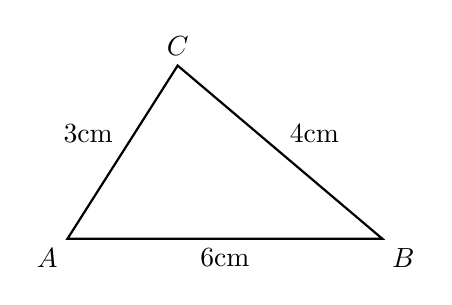
\begin{tikzpicture}[scale=1]
\coordinate (A) at (0,0); \coordinate (B) at (4,0); \coordinate (C) at (1.4,2.2);
\draw[thick] (A)--(B)--(C)--cycle;
\node[below] at ($(A)!0.5!(B)$) {$6\mathrm{cm}$};
\node[above left] at ($(A)!0.5!(C)$) {$3\mathrm{cm}$};
\node[above right] at ($(B)!0.5!(C)$) {$4\mathrm{cm}$};
\node[below left] at (A) {$A$}; \node[below right] at (B) {$B$}; \node[above] at (C) {$C$};
\end{tikzpicture}
\end{document}
